\clearpage
\section{Extended Intervention Trajectories}
\label{supp:extended-interventions}
Figures~\ref{fig:app-updates}--\ref{fig:app-selected} retain complete
post-intervention update histories, intervention activity, and selected
representation trajectories. The applied increments differ from raw
gradients; nominal coefficients do not match effective intervention
strength. The selected conventional settings illustrate contrasting
behaviors, rather than rank each family's best setting. Section S5
retains the complete matched outcomes.

\begin{figure}[H]
\centering
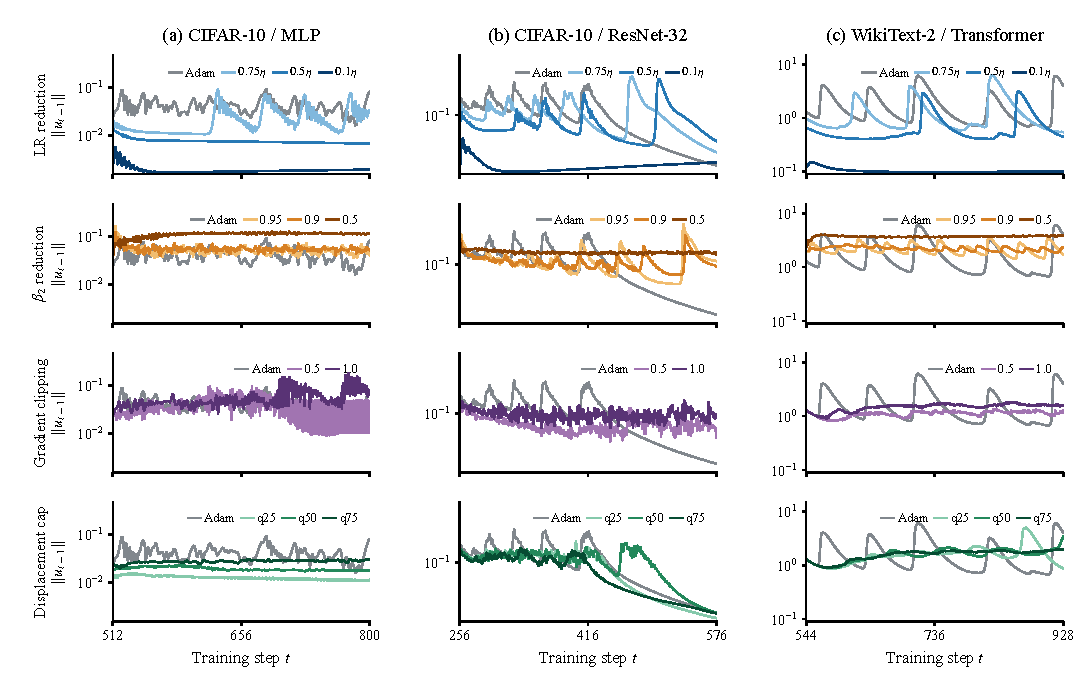
\includegraphics[width=\linewidth,height=.78\textheight,keepaspectratio]{figures/a01-matched-applied-updates.pdf}
\caption{Actual applied update norms for all matched interventions. Rows correspond to immediate learning-rate reduction, late $\beta_2$ reduction, global gradient clipping, and distributed displacement caps. Gray is the same unchanged-Adam control in every row. All post-start updates are retained without smoothing; the log scale is shared across families within each model. Update $u_{t-1}$ is placed at its completed-state endpoint $t$.}
\label{fig:app-updates}
\end{figure}

\clearpage
\begin{figure}[H]
\centering
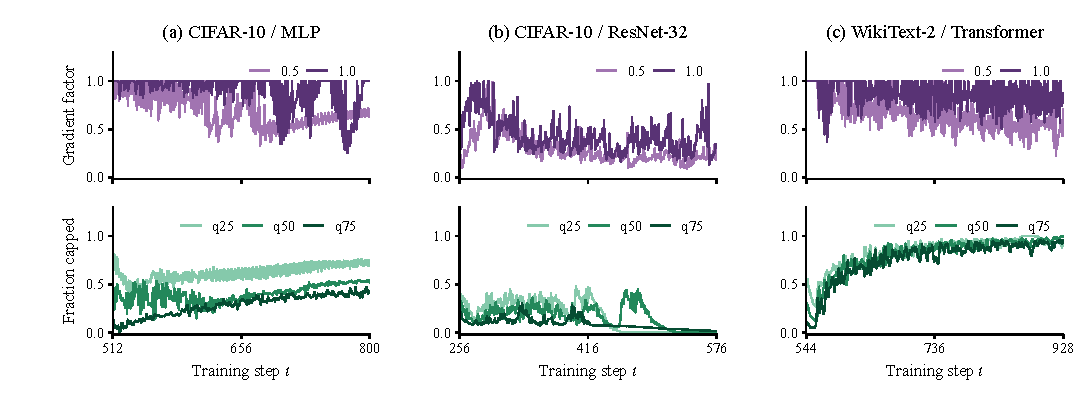
\includegraphics[width=\linewidth,height=.78\textheight,keepaspectratio]{figures/a02-matched-controller-activity.pdf}
\caption{Controller activity over the same complete windows. Top: multiplicative factor retained by global gradient clipping before Adam; one means no clipping. Bottom: fraction of targeted units whose proposed increments are scaled by the displacement cap, pooled over all targeted sites; zero means no units capped. A clipping factor is not an Adam update-retention factor. All values are aligned with completed updates and unsmoothed.}
\label{fig:app-activity}
\end{figure}

\clearpage
\begin{figure}[H]
\centering
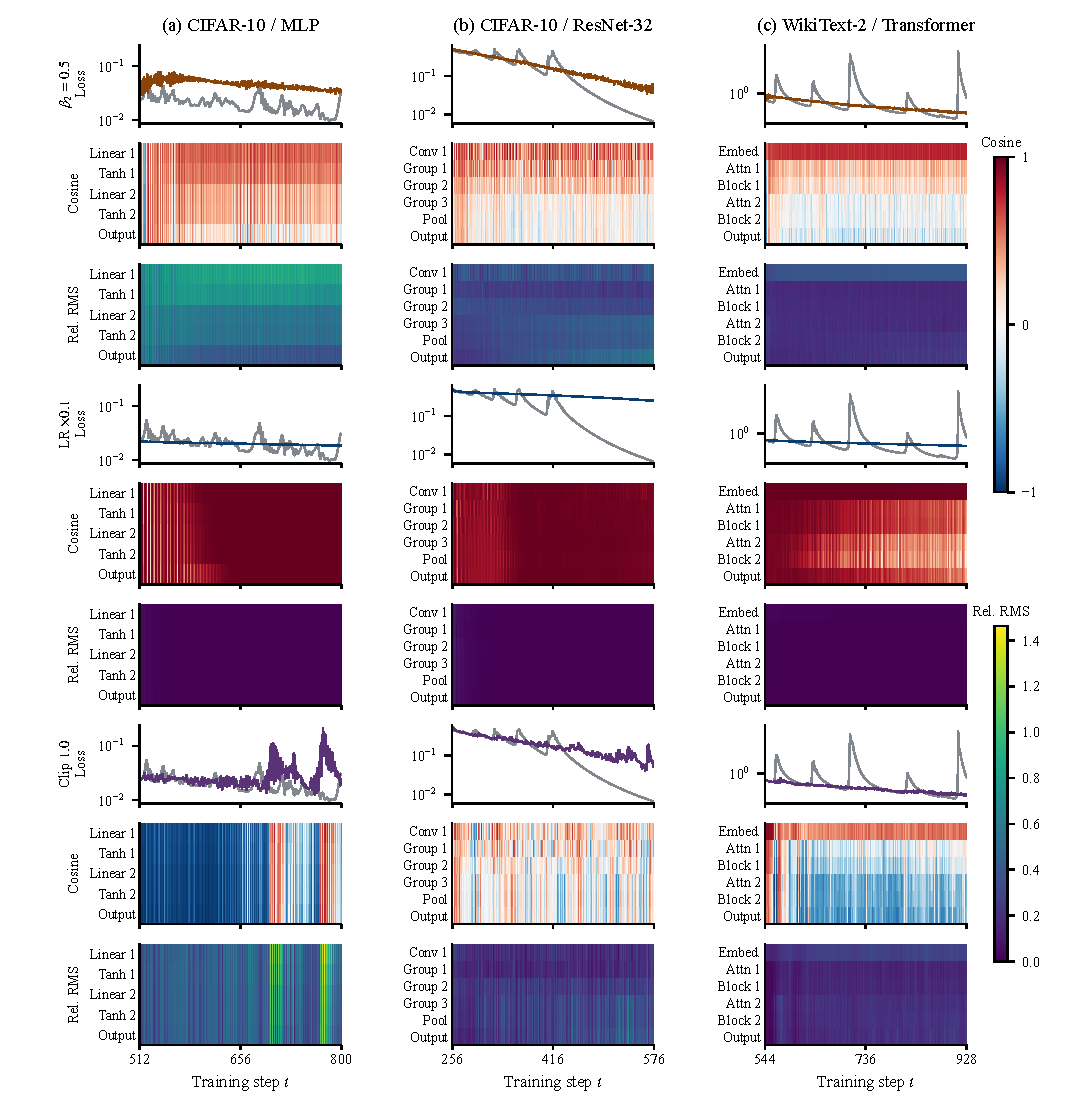
\includegraphics[width=\linewidth,height=.78\textheight,keepaspectratio]{figures/a03-selected-intervention-motion.pdf}
\caption{Selected conventional interventions across the three models: $\beta_2=0.5$ (top block), LR $\times0.1$ (middle), and clip threshold 1.0 (bottom). Each block shows full training loss, consecutive representation-change cosine, and relative RMS displacement. Gray loss curves are unchanged Adam; colored curves and all heatmaps belong to the selected intervention. No Adam heatmaps are repeated. Log-loss limits are shared across the three blocks within each model. RMS uses each site's unchanged-Adam maximum as a common denominator, with one color scale across all selected settings and models; values above one exceed that baseline maximum. Every post-start change is retained, without smoothing, layer averaging, or peak markers. Sites match the main paper's representation-motion figure.}
\label{fig:app-selected}
\end{figure}
\clearpage
